\section{Wstęp teoretyczny}
\label{sec:TheoreticalIntroduction}

\newcommand{\equ}[1]{{\Large #1}}

\subsection{Stwardnienie rozsiane}
\subsubsection{Opis choroby} 
\label{sec:MSPhenotypes}
Stwardnienie rozsiane (MS \textit{lub} SM) \la{sclerosis multiplex} jest przewlekłą i zapalną chorobą ośrodkowego układu nerwowego (OUN), której częstość występowania w centralnej Europie wynosi od 62 do 128 na 100 000 osób\cite{Kingwell2013} i różni się w zależności od regionu. Powoduje ona uszkodzenie fragmentu tkanki OUN, przez co objawiać się może prawie każdym neurologicznym symptomem. Osoby dotknięte tą chorobą mogą stracić czucie, doświadczać ataków bólowych, tracić wzrok, mieć problem z koordynacją ruchową, mową lub przełykaniem, doświadczać kurczów mięśniowych, prowadzących do utraty chodu bądź niemożności trzymania rzeczy w dłoniach\cite{Gelfand2014}. Ponadto mogą objawić się u nich problemy z szybkością przetwarzania słyszanych informacji i problemy takie jak depresja i niestabilny nastrój\cite{Benedict2020-at}. Nie ma konsensusu naukowego dotyczącego przyczyny choroby, choć wymienia się wpływ środowiskowy i genetyczny. Nie jest znane też lekarstwo pozwalające wyleczyć z MS. Znane są jedynie lekarstwa wstrzymujące rozwój choroby oraz zapobiegające występowaniu objawów klinicznych\cite{Koriem2016}. Choroba jest jednym z najczęstszych powodów niepełnosprawności u młodych osób\cite{Browne2014}.
\par
Można rozróżnić kilka różne fenotypy stwardnienia rozsianego, czyli rodzaje przebiegów. Na podstawie dotychczasowego przebiegu próbuje się określić spodziewaną kontynuację choroby, gdyż ma to duże znaczenie w leczeniu.
Międzynarodowy Komitet Doradczy ds. Badań Klinicznych w Stwardnieniu Rozsianym wyróżnia cztery postacie MS znane jako klasyfikacja Lublina z 2013\cite{Lublin2014-md}. Są to postacie:
\begin{itemize}
    \item Rzutowo-remisyjna (RRMS), charakteryzująca się występowaniem rzutów choroby, po których następuje długi czas remisji, czyli okresu bez wyraźnych objawów klinicznych. 
    \item Wtórnie postępująca (SPMS), często pojawiająca się u osób z pierwotnie stwierdzoną postacią RRMS. Charakteryzuje się tym, że zamiast okresów remisji stopień niepełnosprawności postępuje w sposób ciągły.
    \item Pierwotnie postępująca (PPMS), charakteryzująca się brakiem remisji po stwierdzeniu pierwotnych objawów klinicznych. Choroba postępuje, jednak bez wyraźnych rzutów.
    \item Klinicznie izolowany zespół (CIS), charakteryzujący się objawami klinicznymi, w postaci co najmniej 24 godzinnego rzutu choroby spowodowanego demielinizacją i jedną lezją na obrazie MRI. Zgodnie z kryterium MacDonalda opisanym w sekcji \ref{sec:MSMacDonald}, CIS nie jest pełną diagnozą. Jedynie u od 30\% do 70\% osób z CIS stwardnienie się rozwija\cite{Miller2005-ex}.
\end{itemize}
Do 2013 roku wyróżniano również postać postępująco-nawrotową, charakteryzującą się rzutami choroby i pomiędzy nimi postępującą niepełnosprawnością. Zgodnie z aktualizacją wspomnianego Komitetu Doradczego ds. Badań Klinicznych w MS, postać ta jest podtypem postaci pierwotnie postępującej, klasyfikowanym jako PP-aktywna\cite{Lublin2014-md}.
\addImage{fig:MS_phenotypes}{src/img/TheoreticalIntroduction/MS_phenotypes.png}{Postacie przebiegu MS}

\subsubsection{Lezje stwardnienia rozsianego}
Diagnoza MS opiera się na wykryciu dużych, zlewających się zmian demielinizacyjnych, zwanych \textit{lezjami}, w istocie białej i szarej OUN. Powstały one na skutek procesu demielinizacji, będącego trwałym i całkowitym uszkodzeniem oligodendrocytów formujących osłonę  mielinową w OUN, co z kolei jest przyczyną częściowego uszkodzenia aksonów w komórce nerwowej. Same lezje w istocie składają się z limfocytów T, limfocytów B i plazmocytów osadzających się w miejscach zmian demielinizacyjnych. Wraz z czasem, miejsca te się łączą i rozszerzają się na swych granicach do zdrowej tkanki tworząc widoczne na obrazie MRI zmiany\cite{Lassmann2018-fl}. 
\par 
W praktyce klinicznej zmiany te obserwuje diagnosta i oznacza. Nie rozróżnia jednak uszkodzenia według ich pochodzenia, stąd nie może z całą pewnością określić, że zmiany widoczne na skanie MRI są wynikiem MS. Proces oznaczenia lezji postuluje się wykonać w niniejszej pracy za pomocą sztucznych sieci neuronowych. 
\addImage{fig:MRILesions}{src/img/TheoreticalIntroduction/lesions.png}{Na lewym obrazie MRI mózgu, na prawym obrazie oznaczenie lezji}


\subsubsection{Kryterium diagnostyczne MacDonalda}
\label{sec:MSMacDonald}
Kryterium MacDonalda jest standardowym kryterium diagnostycznym MS, zastępującym wcześniej używane kryterium Poser'a i Schumacher'a. Uznaje się, że kryterium MacDonalda przyczynia się do wzrostu czułości diagnostyki MS, bez zwiększenia swoistości\cite{Ntranos2016-yr}. Wykorzystuje się w nim pojęcie rozpowszechnienia choroby w czasie (DIT) \en{dissemination in time} oraz w przestrzeni (DIS) \en{dissemination in space}. Pierwsze oznacza, że uszkodzenia pojawiły się w różnym czasie, a drugie, że dotyczyło innych części układu nerwowego. Jedną z przesłanek wykorzystywaną do stwierdzenia MS według kryterium MacDonalda, są lezje obserwowane na obrazie MRI. Szczegółowy opis kryteriów nie będzie przedstawiany jako nieistotny w kontekście problematyki pracy.


\subsection{Klasyfikatory binarne}
\subsubsection{Pojęcie klasyfikacji}
Klasyfikacją nazywa się zbiór par punktów $X \times Y = \{(x_i, y_i)\}^N_{i=1}$, gdzie $x_i \in \mathbb{R}^D$ jest wektorem cech danego przykładu, a $y_i \in \{1, \dots, K\}$ określa jego klasę. Funkcję odwzorowującą dowolny zbiór $X$ na $Y$ określa się mianem klasyfikatora i możemy ją przedstawić jako $c : \mathbb{R}^D \rightarrow \{1, \dots, K\}$, gdzie $\mathbb{R}^D$ jest zbiorem możliwych obserwacji, a $\{1, \dots, K\}$ jest zbiorem klas\cite{matematyk2022-fh}. Funkcję tą nazywa się klasyfikatorem. 
\par 
W przypadku segmentacji binarnej możemy założyć, że $X$ jest wektorem pikseli na obrazie, a $Y = \{0,1\}$ jest zbiorem klas, a sam proces segmentacji jest procesem klasyfikacyjnym na każdym pikselu obrazu. 

\subsubsection{Problem klasyfikacji niezbalansowanej}
W przypadku większości modeli klasyfikatorów zakłada się niejawnie równoliczność klas, co potencjalnie powoduje, że klasyfikator skupi się na poprawnym zaklasyfikowaniu klasy większościowej, jednocześnie ignorując klasę mniejszościową, gdyż wartości funkcji kosztu oraz metryki ewaluacyjne związane z błędną klasyfikacją małej liczby przypadków jest mała. W przypadku dużej dysproporcji mówi się o niezbalansowaniu klas i często występuje w problemach medycznych, gdzie jednostka chorobowa jest wykrywana stosunkowo rzadko lub w problematyce rozliczeniowej w problemie wykrywania przez banki niewielkiej liczby fałszywych transakcji. Wszystko to sprawia, że uczenie i ewaluacja klasyfikatorów jest trudna. Stosuje się dwa podejścia do rozwiązania tego problemu w procesie tworzenia klasyfikatora\cite{matematyk2022-fh}:
\begin{itemize}
    \item \textbf{Losowanie} Polega na takim dobraniu zbioru treningowego, aby proporcja klas była równa. Można dodać kopie klasy mniejszościowej do zbioru treningowego, zmniejszając dysproporcję klas. Technika ta nazywana jest \textit{oversampling}. Można też dokonać losowania podzbioru klasy większościowej osiągając podobny efekt. Tą technikę nazywa się \textit{undersampling} i można ją zastosować tylko przy wtedy, gdy dostateczna jest ilość elementów w klasie mniejszościowej, ze względu na wymagania procesu uczenia.  
    \item \textbf{Wagowanie} Polega na przypisaniu do każdego punktu klas mniejszościowej oraz większościowej  wagi danej odpowiednio wzorami:
    \par \[w_i=\mathrm{\frac{|X_{major}|}{|X_{minor}|}} \quad \mathrm{ oraz } \quad  w_i=1\]
    \par
    W przypadku funkcji ewaluacyjnej lub kosztu modelu klasyfikatora $\sum {C_{\Phi}(x_i,y_i)}$, gdzie $ C_{\Phi}(x_i,y_i)$ jest kosztem błędnego zaklasyfikowania pojedynczego elementu, wagowanie powyższej funkcji wyraża się wzorem:
    \par
    \[\sum_{i} w_iC_{\Phi}(x_i,y_i)\]

\end{itemize}

\subsection{Ewaluacja klasyfikatorów binarnych}
\label{sec:evaluation}
Ewaluacja segmentacji binarnej wymaga zastosowania szeregu metryk, jako pewnych statystyk świadczących o różnicach pomiędzy jej rezultatem a wartością rzeczywistą, a w praktyce standardem referencyjnym. Metryki te mogą w swojej istocie odpowiadać na konkretnie, z analitycznego punktu widzenia, określony problem. Każdą bowiem segmentację można rozumieć jako problem klasyfikacji, w przypadku segmentacji rynku w pojęciu nauk ekonomicznych jako podzielenie tegoż na klasy, a w przypadku segmentacji obrazów jako przypisywanie wszystkich pikseli do konkretnych klas. W tym znaczeniu, problem klasyfikacji binarnej jest tożsamy z problemem segmentacji i można stosować jej metryki do problemów z zakresu segmentacji. 
% W procesie uczenia maszynowego sieć jest warunkowana przez minimalizację wartości funkcji kosztu. 
\subsubsection{Macierz błędów i metryki}
\label{sec:confusion-matrix-and-metrics}
\begin{table}[H]
    \centering
    \caption{Macierz błędów}
    \begin{tblr}{
        hlines,
        vlines,
        colspec={QQQQ},
        cells={mode=text, halign=c, valign=m},
        cell{1}{3}={mode=text,font=\bfseries},
        cell{3}{1}={mode=text,font=\bfseries},
    }
        \SetCell[c=2,r=2]{m} & & \SetCell[c=2]{} Klasa predykowana\\
        & & Pozytywna & Negatywna \\
        \SetCell[r=2]{m} \shortstack{Klasa  \\ rzeczywista}& Pozytywna & Prawdziwie pozytywna (TP) & Fałszywie negatywna (FN)\\
        & Negatywna & Fałszywie pozytywna (FP)&Prawdziwie negatywna (TN) \\
    \end{tblr}
    \label{tab:ConfusionMatrix}
\end{table}

Każdą klasyfikację można określić jako prawdziwą (T) jeśli jest zgodną z wartością rzeczywistą oraz fałszywą (F) jeśli zgodną nie jest. Klasy binarnego klasyfikatora określa się jako (P) oraz (N) i dla wygody przyjęto dla nich nazewnictwo odpowiednio "pozytywne" i "negatywne". W ten sposób powstają cztery kombinacje: 
\begin{itemize}
    \item \textbf{Prawdziwie pozytywna (TP)} \en{true positive}, oznaczająca zbiór elementów prawidłowo zaklasyfikowanych do klasy "pozytywne".
    \item \textbf{Fałszywie pozytywna (FP)} \en{false positive}, oznaczająca zbiór elementów nieprawidłowo zaklasyfikowanych do klasy "pozytywne".
    \item \textbf{Prawdziwie negatywna (TN)} \en{true negative}, oznaczająca zbiór elementów prawidłowo zaklasyfikowanych do klasy "negatywne".
    \item \textbf{Fałszywie negatywna (FN)} \en{false negative}, oznaczająca zbiór elementów nieprawidłowo zaklasyfikowanych do klasy "negatywne".
\end{itemize} 

\par W statystyce częstościowej przyjęło się określać predykcję FP jako \textbf{błąd I rodzaju}, a predykcję FN jako \textbf{błąd II rodzaju}. Pierwszy polega na odrzuceniu prawdziwej hipotezy zerowej a oszacowanie prawdopodobieństwa jego błędu nazywa się \textit{poziomem istotności testu}. Drugi polega na nieodrzuceniu fałszywej hipotezy zerowej.

Liczba elementów w podzbiorach "pozytywnych" i "negatywnych" jest równa liczbie wszystkich elementów zbioru, oraz zbiory te są wzajemnie rozłączne. Z tak ustanowionej macierzy można wyznaczyć wartości brzegowe, razem z wartościami z samej macierzy generujące szereg wskaźników. Na podstawie liczności TP, FP, FN oraz TP określa się szereg metryk klasyfikacji obrazu.

Te wskaźniki przedstawia się poniżej:

\begin{itemize}
    \item[$\blacksquare$] \textbf{Precyzja} \en{positive predictive value}
    \par Wskaźnik określa stosunek dobrze zaklasyfikowanych elementów pozytywnych do ilości wszystkich zaklasyfikowanych elementów pozytywnych. Metryka tym samym określa jakość predykcji pozytywnych. 
    \par 
    \equ{$ \mathrm{PPV = \frac{|TP|}{|TP|+|FP|}}$}

    \item[$\blacksquare$] \textbf{Wartość predykcyjna ujemna} \en{negative predictive value}
    \par Wskaźnik określa stosunek dobrze zaklasyfikowanych elementów negatywnych do ilości wszystkich zaklasyfikowanych elementów negatywnych. Metryka tym samym określa jakość predykcji negatywnych. 
    \par 
    \equ{$ \mathrm{NPV = \frac{|TN|}{|TN|+|FN|}}$}
    
    \item[$\blacksquare$] \textbf{Dokładność} \en{accuracy}
    \par Wskaźnik określa stosunek dobrze zaklasyfikowanych elementów do ilości wszystkich  elementów zbioru. Ma swoje liczne wady w klasyfikacji medycznej, gdyż istotniejsza z punktu widzenia diagnozy medycznej jest właściwa klasyfikacja osób chorych, a metryka ta tego nie uwzględnia. Wady te nazwane zostały paradoksem dokładności \en{accuracy paradox}.
    \par 
    \equ{$ \mathrm{ACC = \frac{|TP|+|TN|}{|TP|+|FP|+|TN|+|FN|}}$}

    \item[$\blacksquare$] \textbf{Zbalansowana dokładność} \en{balanced accuracy}
    \par W przypadku problemów niezbalansowanych, w których liczba przypadków jednej klasy znacznie przewyższa liczbę drugiej klasy, możliwe jest przy niepoprawnej klasyfikacji otrzymanie dobrej miary dokładności, przypisując wszystkie elementy do klasy większościowej. Zbalansowana dokładność jest średnią z przewidywania obu klas.
    \par 
    \equ{$ \mathrm{BACC = \frac{1}{2}\bigg(\frac{|TP|}{|TP|+|FN|}+\frac{|TN|}{|TN|+|FP|}\bigg)}$}
    
    \item[$\blacksquare$] \textbf{Czułość} \en{recall, sensitivity, true positive ratio}
    \par Wskaźnik określa jaki jest udział dobrych predykcji pozytywnych wśród wszystkich przypadków pozytywnych. W przypadku badań medycznych metryka posiada duże znaczenie, jako, że marginalizuje fałszywie pozytywną diagnozę, natomiast fałszywie negatywne klasyfikacje mają na nią duży wpływ. Innymi słowy dopuszcza możliwość pomyłki fałszywego zdiagnozowania pacjenta jako chorego, ale nie dopuszcza pomyłki błędnego zaklasyfikowania osoby chorej.
    \par 
    \equ{$ \mathrm{TPR = \frac{|TP|}{|TP|+|FN|}}$}

    \item[$\blacksquare$] \textbf{Swoistość} \en{specificity, true negative rate}
    \par Metryka określająca prawdopodobieństwo prawdziwie negatywnej predykcji wśród wszystkich rzeczywiście negatywnych elementów.
    \par
    \equ{$\mathrm{TNR=\frac{|TP|}{|TP|+|FP|}}$}
    
    \item[$\blacksquare$] \textbf{Współczynnik Sørensen'a–Dice'a}
    \par Inaczej współczynnik F\textsubscript{1}. Wskaźnik jest istotnie średnią harmoniczną precyzji i czułości.  
    \par
    \equ{$ \mathrm{F_1 = \frac{2\cdot{}|TP|}{2|TP|+|FP|+|FN|} = 2\frac{PPV\cdot{}TPR}{PPV+TPR}}$}

    \item[$\blacksquare$] \textbf{Współczynnik F\textsubscript{$\beta$}}
    \par Wskaźnik jest uogólnieniem wskaźnika F\textsubscript{1}, pozwalającym na zmienienie wagi precyzji i czułości.
    \par
    \equ{$ \mathrm{F_\beta = \frac{\big(1+\beta^2\big)\cdot{}|TP|}{\big(1+\beta^2\big)|TP|+\beta^2|FN|+|FP|} = \big(1+\beta^2\big)\frac{PPV\cdot{}TPR}{\beta^2 PPV+TPR}}$}

    \item[$\blacksquare$] \textbf{Kappa Cohena}
    \par Wskaźnik jest współczynnikiem rzetelności dwukrotnych pomiarów jednej nominalnej i zależnej zmiennej. Przyjmuje wartości z przedziału $[-1,1]$.
    \par
    \equ{$ \mathrm{\kappa = \frac{2\cdot{}\big(|TP|\cdot{}|TN|-|FN|\cdot|FP|\big)}{\big(|TP|+|FP|\big)\cdot{}\big(|FP|+|TN|\big)+\big(|TP|+|FN|\big)\cdot{}\big(|FN|+|TN|\big)}}$}

    \item[$\blacksquare$] \textbf{Współczynnik korelacji Matthews} \en{mean square contingency}
    \par Inaczej współczynnik fi. Wskaźnik jest właściwie współczynnikiem korelacji liniowej Pearsona dla dwóch nominalnych i dychotomicznych zmiennych. 
    \par
    \equ{$ \mathrm{MCC = \phi = \frac{|TP|\cdot{}|TN|-|FN|\cdot|FP|}{\sqrt{\big(|TP|+|FP|\big)\big(|FP|+|TN|\big)\big(|TP|+|FN|\big)\big(|FN|+|TN|\big)}}}$}

    \item[$\blacksquare$] \textbf{Indeks Jaccarda}
    \par Indeks Jaccarda wyznacza ilość prawdziwie pozytywnych predykcji do wszystkich predykcji z wyłączeniem predykcji prawdziwie negatywnych. Tym samym indeks ten ma swoją wartość w przypadku niezbalansowanych danych, gdy zbiór elementów negatywnych jest dużo większy niż pozytywnych. 
    \par
    \equ{$\mathrm{J=\frac{|TP|}{|TP|+|FP|+|FN|}}$}

    \item[$\blacksquare$] \textbf{Indeks P\textsubscript{4}}
    \par
    Metryka P\textsubscript{4} została stworzona jako odpowiedź na krytykę metryki F\textsubscript{1}\cite{sitarz2022extending}.
    \par
    \equ{$\mathrm{P_4=\frac{4\cdot{}|TP|\cdot{}|TN|}{4\cdot{}|TP|\cdot{}|TN|+\big(|TP|+|TN|\big)\big(|FP|+|FN|\big)}}$}

    \item[$\blacksquare$] \textbf{Dystans Hamminga}
    \par Metryka określa to ile elementów predykcji jest różnych od wartości rzeczywistej, tym samym, w klasyfikacji binarnej, będąca w istocie wagą Hamminga, czyli licznością nie-zerowego zbioru, odniesioną do wyniku operacji XOR przeprowadzonej na zbiorach. \cite{Warren2012-lw}
    \par
    \equ{$\mathrm{H = \frac{|FP|+|FN|}{|TP|+|FP|+|TN|+|FN|}}$}

    \item[$\blacksquare$] \textbf{ROC} \en{receiver operating characteristic}
    \par
    \begin{minipage}{0.4\linewidth}
        Krzywa ROC ilustruje zdolność diagnostyczną binarnego systemu klasyfikatora, gdy jego próg odcięcia jest zmienny. Na osi $x$ oznacza się wartość czułości a na osi $y$ oznacza się wartość 1-swoistość. Korzystając z krzywej można określić poziom odcięcia $p$, dla którego dokładnie określona jest miara czułości lub swoistości. Ma swoje wady w ewaluacji danych silnie niezbalansowanych\cite{Saito2015-vf}. Krzywą ROC przedstawiono na rys. \ref{fig:ROCcurve}. 
        \vspace{0.4\linewidth}
    \end{minipage}
    \begin{minipage}{0.6\linewidth}
    
        \begin{figure}[H]
        \centering
            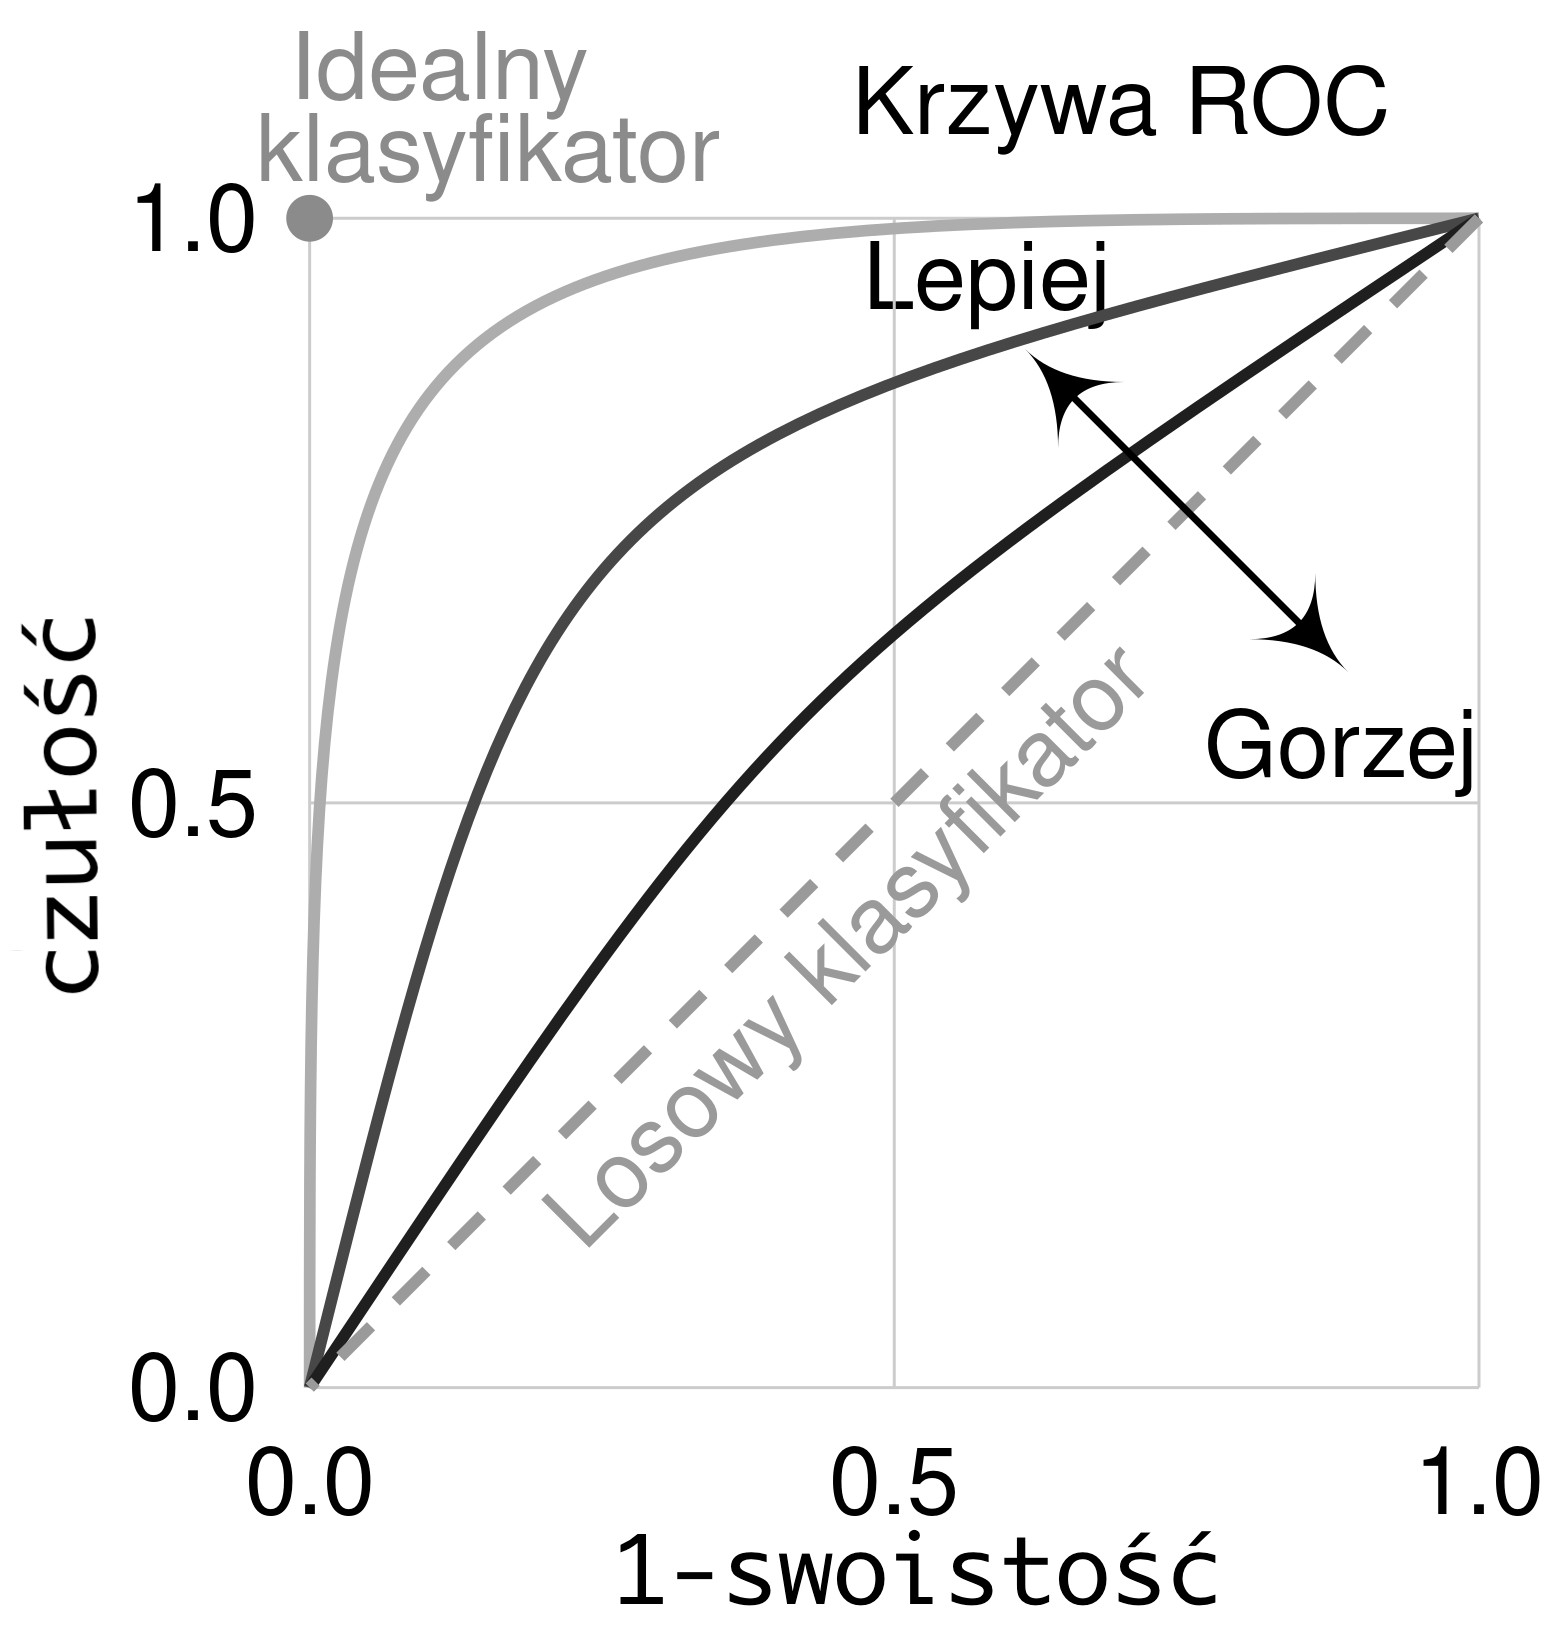
\includegraphics[width=0.9\linewidth]{src/img/TheoreticalIntroduction/Roc_curve_gs.png}
            \caption{Krzywa ROC}
            \label{fig:ROCcurve}
        \end{figure}    
    \end{minipage}


    \item[$\blacksquare$] \textbf{AUC} \en{area under ROC curve}
    \par
    Metrykę wyznacza obszar pod krzywą ROC. Wartość ta nie zależy od progu odcięcia i ilustruje prawdopodobieństwo, że klasyfikator nada losowo wybranemu przykładowi pozytywnemu $x_1$ wyższą wartość niż losowo wybranemu przykładowi negatywnemu $x_2$, czyli $P\big(f\big(x_1\big) > f\big(x_2\big)\big)$\cite{matematyk2022-fh}. Miarę AUC stosuje się w problemach niezbalansowanych.
    
\end{itemize}





\subsection{Sztuczne sieci neuronowe}
\label{sec:ann}
Sztuczne sieci neuronowe to grupa modeli, złożonych z wzajemnie połączonych węzłów zwanymi neuronami. Każdy neuron może transmitować sygnał do innych neuronów z którymi jest połączony, a wpływ na sygnał przekazywany ma waga połączenia. W pewien sposób model odwzorowuje biologiczne neurony i połączenia między aksonami, synapsami i dendrytami. W uproszczeniu, sieć neuronowa formuje transformację $\Phi:\mathbb{R}^D\rightarrow \mathbb{R}^N$\cite{matematyk2022-fh}. 
\par
Zaletą sieci neuronowych jest to, że są użyteczne w rozwiązywaniu problemów z którymi inne, tradycyjne metody sobie nie radzą. Ponadto potrafią w miarę dobrze rozwiązywać dokładnie te problemy, które dla ludzi są łatwe\cite{Karnga1999}. W poniższym rozdziale omówione zostaną jedynie \textbf{sieci jednokierunkowe} \en{feedforward neural network} jako, że ten rodzaj sieci jest wykorzystywany w niniejszej pracy. Inne rodzaje, jak rekurencyjne sieci neuronowe, bądź samoorganizujące się mapy nie będą omawiane. 

\subsubsection{Sztuczny neuron}
\label{sec:ArtificialNeuron}
Sztuczny neuron jest funkcją, która w bardzo uproszczony sposób modeluje biologiczny neuron. Neuron przyjmuje na wejście co najmniej jeden sygnał. Wszystkie sygnały wejścia są sumowane oraz przepuszczone przez nieliniową funkcję aktywacji i propagowane do następnych neuronów\cite{krenker2011introduction}. 
\addImage{fig:neuron}{src/img/TheoreticalIntroduction/neuron.png}{Reprezentacja sztucznego neuronu}
\par
Wyjście z neuronu można analitycznie ująć w następujący sposób:
\par
\[y_k=\phi\bigg(\sum_{j=0}^m w_{kj}x_j\bigg)\]
gdzie $\phi$ jest funkcją aktywacji, $w_{kj}$ wagami, a $x_i$ sygnałem wejściowym.
 \par Tym samym na neuron składają się wagi połączeń do niego dołączonych, wyraz wolny (próg) oraz funkcja aktywacji. W momencie podania sygnału $x_j$ obliczyć można pobudzenie neuronu, czyli sygnał na wyjściu neuronu. Schemat neuronu zaprezentowano na rys. \ref{fig:neuron}.
 

 \subsubsection{Funkcje aktywacji}
  \par Przyjęło się, że \textbf{funkcja aktywacji} węzła sieci neuronowej (neuronu) musi być różniczkowalna, jako że typowe metody optymalizacyjne, opisane w rozdziale \ref{sec:optimization}, wymagają tej własności funkcji w procesie aktualizacji wag. Ponadto w większości problemów wymaga się, żeby funkcja aktywacji była nieliniowa, gdyż złożenie funkcji liniowych jest funkcją liniową i nie nadaje się do rozwiązywania nieliniowych problemów. Już w 1989 roku wykazano, że złożenie nieliniowych funkcji sigmoidalnych może aproksymować dowolną funkcję\cite{cybenko1989approximation}.
  \par
 Wśród najpopularniejszych funkcji aktywacji wymienia się:
 \par
\newcolumntype{M}{>{\centering\arraybackslash}m{\dimexpr.45\linewidth-2\tabcolsep}}
\newcolumntype{L}{>{\centering\arraybackslash}m{\dimexpr.25\linewidth-2\tabcolsep}}


\begin{longtable}[p]{|L|M|L|}
\caption{Funkcje aktywacji} \label{tab:activation-functions}\\
\hline
\textbf{Funkcja} & \textbf{Wzór} & \textbf{Wykres} \\
\hline
\endfirsthead

\multicolumn{3}{c}%
{{\tablename\ \thetable{} -- Kontynuacja z poprzedniej strony}} \\
\hline
\textbf{Funkcja} & \textbf{Wzór} & \textbf{Wykres} \\
\hline
\endhead

\hline \multicolumn{3}{|r|}{{Kontynuacja na następnej stronie}} \\ \hline
\endfoot

\hline
\endlastfoot

Tożsamość & $\text{Id}(x) = x$ & 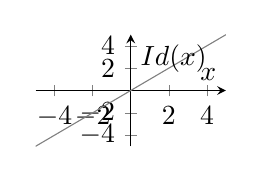
\begin{tikzpicture}
    \begin{axis}[width=4cm, height=3cm, axis lines=middle, xlabel=$x$, ylabel=$\text{Id}(x)$, samples=100]
        \addplot[gray, domain=-5:5] {x};
    \end{axis}
\end{tikzpicture} \\
\hline
Skok Jednostkowy & $\text{Skok}(x) = \begin{cases} 0 & \text{if } x < 0 \\ 1 & \text{if } x \geq 0 \end{cases}$ & 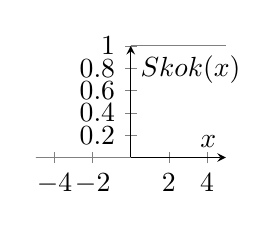
\begin{tikzpicture}
    \begin{axis}[width=4cm, height=3cm, axis lines=middle, xlabel=$x$, ylabel=$\text{Skok}(x)$, samples=100]
        \addplot[gray, domain=-5:0, forget plot] {0};
        \addplot[gray, domain=0:5] {1};
    \end{axis}
\end{tikzpicture} \\
\hline
Sigmoida & $\sigma(x) = \frac{1}{1 + e^{-x}}$ & 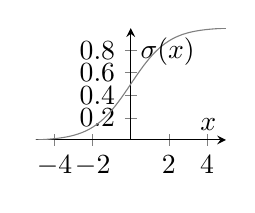
\begin{tikzpicture}
    \begin{axis}[width=4cm, height=3cm, axis lines=middle, xlabel=$x$, ylabel=$\sigma(x)$, samples=100]
        \addplot[gray, domain=-5:5] {1/(1+exp(-x))};
    \end{axis}
\end{tikzpicture} \\
\hline
Tangens Hiperboliczny (tanh) & $\tanh(x) = \frac{e^{x} - e^{-x}}{e^{x} + e^{-x}}$ & 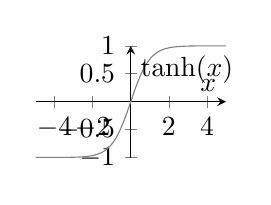
\begin{tikzpicture}
    \begin{axis}[width=4cm, height=3cm, axis lines=middle, xlabel=$x$, ylabel=$\tanh(x)$, samples=100]
        \addplot[gray, domain=-5:5] {(exp(x)-exp(-x))/(exp(x)+exp(-x))};
    \end{axis}
\end{tikzpicture} \\
\hline
ReLU & $\text{ReLU}(x) = \max(0, x)$ & 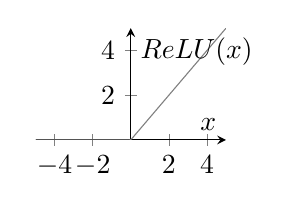
\begin{tikzpicture}
    \begin{axis}[width=4cm, height=3cm, axis lines=middle, xlabel=$x$, ylabel=$\text{ReLU}(x)$, samples=100]
        \addplot[gray, domain=-5:5] {max(0,x)};
    \end{axis}
\end{tikzpicture} \\
\hline
GELU & $\text{GELU}(x) = \frac{1}{2}x\left(1 + \tanh\left(\sqrt{\frac{2}{\pi}}(x + 0.044715x^3)\right)\right)$ & 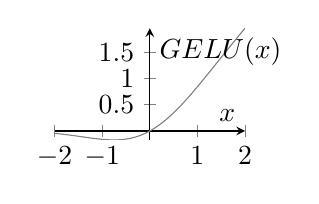
\begin{tikzpicture}
    \begin{axis}[width=4cm, height=3cm, axis lines=middle, xlabel=$x$, ylabel=$\text{GELU}(x)$, samples=100]
        \addplot[gray, domain=-2:2] {0.5*x*(1 + tanh(sqrt(2/pi)*(x + 0.044715*x^3)))};
    \end{axis}
\end{tikzpicture} \\
\hline
ELU & $\text{ELU}(x) = \begin{cases} x & \text{if } x \geq 0 \\ \alpha (e^{x} - 1) & \text{if } x < 0 \end{cases}$ & 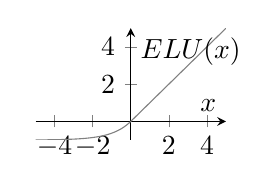
\begin{tikzpicture}
    \begin{axis}[width=4cm, height=3cm, axis lines=middle, xlabel=$x$, ylabel=$\text{ELU}(x)$, samples=100]
        \addplot[gray, domain=-5:5] {ifthenelse(x>=0,x,1*(exp(x)-1))};
    \end{axis}
\end{tikzpicture} \\
\hline
Leaky ReLU & $\text{Leaky ReLU}(x) = \begin{cases} x & \text{if } x \geq 0 \\ \alpha x & \text{if } x < 0 \end{cases}$ & 
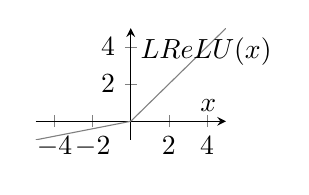
\begin{tikzpicture}
    \begin{axis}[width=4cm, height=3cm, axis lines=middle, xlabel=$x$, ylabel=$\text{L ReLU}(x)$, samples=100]
        \addplot[gray, domain=-5:5] {ifthenelse(x>=0,x,0.2*x)};
    \end{axis}
\end{tikzpicture} \\
\hline
Rozkład Gaussa & $\text{Gauss}(x) = e^{-x^2}$ & 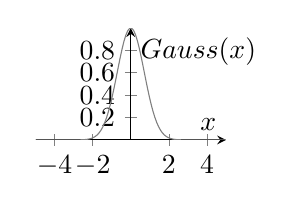
\begin{tikzpicture}
    \begin{axis}[width=4cm, height=3cm, axis lines=middle, xlabel=$x$, ylabel=$\text{Gauss}(x)$, samples=100]
        \addplot[gray, domain=-5:5] {exp(-x^2)};
    \end{axis}
\end{tikzpicture} \\
\hline
Softplus & $\text{Softplus}(x) = \ln(1+e^x)$ & 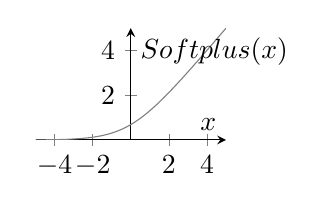
\begin{tikzpicture}
    \begin{axis}[width=4cm, height=3cm, axis lines=middle, xlabel=$x$, ylabel=$\text{Softplus}(x)$, samples=100]
        \addplot[gray, domain=-5:5] {ln(1+exp(x))};
    \end{axis}
\end{tikzpicture} \\
\hline

\end{longtable}

 

\subsection{Perceptrony wielowarstwowe}
\label{sec:NNArchitecture}
Podstawową i najprostszą jednokierunkową siecią neuronową jest perceptron wielowarstwowy MLP \en{multilayer perceptron}. 
Budowę tej sieci konstytuują połączone ze sobą neurony  organizowane w pełni połączone warstwy. Każde dwie sąsiadujące warstwy tworzą ze sobą skierowany i pełny graf dwudzielny z wagami, w którym węzły reprezentowane są przez neurony. Każdy neuron odbiera sygnał od neuronów połączonych z nim w poprzedniej warstwie, a następnie z wykorzystaniem nieliniowej funkcji wyznacza wyjście do kolejnej warstwy na podstawie sumy wejść. Połączenia zwykle mają wagi aktualizowane w procesie uczenia, które wpływają na wartość przepuszczanego sygnału. Sygnał na wejściu sieci jest modyfikowany przez nią, a następnie zwracany w ostatniej warstwie. Przyjęło się nazywać sieci neuronowe \textit{głębokimi} gdy posiadają co najmniej dwie \textit{ukryte} warstwy. Schemat MLP przedstawiono na rys. \ref{fig:MLP}.

\par
Perceptron wielowarstwowy można opisać formalnie za pomocą złożenia funkcji opisującej przekształcenia dokonywane na kolejnych warstwach.
Formalnie, każdą warstwę ukrytą zdefiniować można funkcją w sposób następujący:
\[f_i(x_{i-1})=\sigma(W_i^Tx_{i-1}+b_i)\]
gdzie $\sigma : \mathbb{R} \rightarrow \mathbb{R}$ jest nieliniową funkcją aktywacji, $b_i$ jest wektorem wyrazów wolnych, a $W_i$ macierzą wag. 
\par
Sieć wówczas jest złożeniem funkcji $f_i$ każdej warstwy ukrytej:
\[\phi=f_k\circ \dots \circ f_1\]

A jej warstwa wyjściowa definiowana jest przez wzór:
\[\hat{y}=W^T_o\phi(x)+b_o\]
gdzie $\hat{y}$ odpowiedzią sieci\cite{matematyk2022-fh}. 
\addImage{fig:MLP}{src/img/TheoreticalIntroduction/mlp.png}{Organizacja sieci MLP}

\subsection{Splotowe sieci neuronowe}
\label{sec:cnn}
Splotowe sieci neuronowe są typem jednokierunkowej sieci neuronowej, w której w procesie uczenia optymalizuje się parametry filtrów. Sieci te zakładają wewnętrzne uporządkowania danych wejściowych. Tym samym silną korelację pomiędzy pobliskimi elementami wejścia\cite{lecun1998gradient}. Szczegóły reprezentacji danych przedstawione są poniżej, w rozdziale \ref{sec:imgRepresentation}.
\subsubsection{Reprezentacja obrazu}
\label{sec:imgRepresentation}
\par
Każdy obraz możemy reprezentować jako pewną macierz, której współczynniki opisują w sposób numeryczny wartość piksela, a wzajemne ułożenie elementów macierzy przenosi informację o rozkładzie pikseli na obrazie. W przypadku podstawowych modeli kolorów takich jak RGB, macierz złożona jest z trzech komponentów odpowiadających barwom R - czerwona, G - zielona, B - niebieska, reprezentowanych przez dodatkowy wymiar, zwany \textit{kanałem}. Uogólnienie macierzy z dwóch na dowolną liczbę wymiarów nazywamy tensorem. W przypadku obrazu w skali szarości obraz przechowywany jest przez jeden kanał\cite{zhong2016overview}. 
\par 
W przypadku uczenia sieci MLP do analizy obrazów, obraz wejściowy poddaje się spłaszczeniu \en{flattening}. W przypadku tensora $H=[h_{ijk}]$, gdzie $i \in \{x \in \mathbb{Z}_+ \ | \ x <h \}$, $j \in \{x \in \mathbb{Z}_+ \ | \ x <w \}$,  $k \in \{x \in \mathbb{Z}_+ \ | \ x <c \}$, gdzie $h,w,c$ wysokość obrazu, szerokość obrazu, ilość kanałów odpowiednio, otrzymuje się wektor o wielkości $L=hwc$.
\addImage{fig:flattening}{src/img/TheoreticalIntroduction/flattening.png}{Spłaszczenie tensora do reprezentacji wektorowej}
\par
Sieci MLP jednak mają istotną wadę w rozwiązywaniu problemów wizji komputerowej. W przypadku nawet małych obrazów wielkości 128x128x3 pojedynczy neuron miałby 49153 parametry (łącznie z wyrazem wolnym). Ponieważ sieć złożona jest z wielu neuronów, ilość parametrów jest olbrzymia. Wraz ze zwiększeniem rozdzielczości obrazu ilość parametrów rośnie w sposób kwadratowy. Problem ten nazwany został przekleństwem wymiarowości. Ponadto spłaszczenie obrazu powoduje zanik łatwych korelacji pomiędzy bliskimi pikselami. W procesie uczenia sieć może się nauczyć takich korelacji, jednak wymaga to wiele czasu i olbrzymiej ilości danych\cite{matematyk2022-fh}. Dlatego współcześnie rzadko korzysta się się z sieci MLP celem analizy obrazu. Lepszym podejściem okazują się sieci splotowe. 


\subsubsection{Filtry splotowe}
\label{sec:convolutionalFilters}
Splot jest przekształceniem zdefiniowanym na dwóch funkcjach:
\[(f*g)(t):=\int_{-\infty}^{\infty}f(\tau)g(t-\tau)d\tau\]
\par
Dyskretny splot, używany często w przekształceniach obrazów, definiuje się wzorem\cite{matematyk2022-fh}:
\[g_{xy}=\sum_{i,j,k}h_{ijk}w_{x+i,y+j,k}\]
gdzie 
$W=[w_{ijk}]$ jest tensorem definiującym filtr. Zazwyczaj wymiary filtra są dużo mniejsze niż wymiary obrazu. Splot zachowuje pierwotną informację przestrzenną. Przedstawiono go na rys. \ref{fig:convolution}.

\addImage{fig:convolution}{src/img/TheoreticalIntroduction/convolution.png}{Działanie filtra splotowego. Filtr W jest przykładany do każdego piksela obrazu H otrzymując nową wartość w pikselu, zależną również od początkowego otoczcenia wyrazu}

\subsubsection{Operacja redukująca}
Operacja redukująca \en{pooling} jest najczęściej przeprowadzana z wykorzystaniem filtrów maksymalizujących, który wydobywa maksymalną aktywację z danego pola percepcji. Wówczas nazywana jest \en{max-pooling}. Filtr maksymalizujący ten można przedstawić w następujący sposób:
\[g_{xy}=\max{h_{x \pm i, y \pm j}}\]
gdzie $I,J$ - wymiary filtra, $i \in I, j \in J$. W przypadku wielu splotowych sieci neuronowych filtr ten stosuje się do wybranych elementów obrazu, redukując tym samym jego wymiary, co przekłada się na zmniejszenie złożoności obliczeniowej w procesie uczenia, ograniczenie liczby parametrów i mniejsze zużycie pamięci, a to z kolei ogranicza nadmierne dopasowanie. Stosuje się do tego krok \en{stride}. Jeśli krok równy jest 2x2 to znaczy że do co drugiego piksela w pionie i poziomie przykłada się filtr. 
Operację redukującą przedstawia się na rys \ref{fig:maxpool}.
\addImage{fig:maxpool}{src/img/TheoreticalIntroduction/maxpool.png}{Operacja redukująca max-pool, z wielkością filtra 2x2 i krokiem 2x2}
\par
Wraz z przykładaniem filtra stosuje się również operację dopełnienia \en{padding}. Ma to na celu rozwiązanie problemu z krańcowymi pikselami do których nie można przyłożyć filtra, bo zakres indeksów wykracza poza zakres obrazu. Stosuje się zazwyczaj tzw. zero-padding, czyli dodaje się odpowiedni margines do obrazu wejściowego złożonego z zer. Stosuje się również czasami no-padding, czyli po prostu ignoruje się przyłożenie filtra do skrajnych pikseli (rys. \ref{fig:maxpool}).




\subsubsection{Architektura sieci splotowych}
W sieciach splotowych optymalizuje się wzorce (parametry filtra), tak aby możliwie dobrze rozwiązywały postawione zadanie. Sieć jest podtypem jednokierunkowych sieci neuronowych więc składa się z warstwy wejściowej, warstw ukrytych i warstwy wyjściowej. Wśród warstw ukrytych znajdują się warstwy splotowe \en{convolutional layars} i redukujące \en{pooling layers}.
\par

\begin{description}
    \item[Warstwa splotowa]  
    Zawiera zestaw filtrów, które przekształcają otrzymany obraz. Parametry filtrów podlegają procesowi uczenia. Po każdej warstwie splotowej otrzymywany jest obraz $H_m$, z których ostatni stanowi wysokopoziomową reprezentację początkowego obrazu. Do wyjścia stosuje się funkcję aktywacji wprowadzającą nieliniowość do procesu. W przypadku klasycznego problemu klasyfikacyjnego obraz rzutuje się do przestrzeni klas. Na wyjściu warstwy otrzymywany jest obraz\cite{matematyk2022-fh}:
    \[H_1=f(H*W_1), \dots, f(H*W_l)\]
    \item[Warstwa redukująca]
    Z wykorzystaniem operacji redukującej, zmniejsza wymiarowość danych, co jest często niezbędne aby zredukować złożoność obliczeniową procesu treningowego. Tym samym warstwa ta pełni rolę próbkowania sygnału wejściowego \en{downsampling}.
\end{description}
\par 

Filtr $W_j$ przyłożony do piksela o indeksie $(i,j)$ obrazu $H$ jest utożsamiany z neuronem, w którym wagi są parametrami filtra. W sieci splotowej wagi neuronu nie są połączone ze wszystkimi neuronami z poprzedniej warstwy, ale z pikselami w ich polach percepcyjnych. Ponieważ wagi są współdzielone, zachodzi redukcja w ilości parametrów sieci w zestawieniu z sieciami w pełni połączonymi jak MLP.
\par
W przetwarzaniu danych splot posiada ważne zalety w zestawieniu z klasycznymi metodami używanymi w sieciach w pełni połączonych. Są to lokalność połączeń, wspólne wartości wag połączeń filtru, a na skutek tego niezmienniczość (ekwiwariancja) względem przesunięcia\cite{osowski2018glkebokie}, a więc i lepszą generalizacja. Najprostszym przykładem ekwiwariancji byłby przykład, kiedy ucząc sieć w zbiorze uczącym, wykrywany obiekt występował tylko na pewnym miejscu obrazu. Dla sieci FC w momencie przedstawienia jej nowej danej z tym samym obiektem, lecz w innym miejscu niż w zbiorze uczącym, rzeczone dwa obiekty są różne. W przypadku sieci splotowych, w których używa się filtrów niezależnych od położenia, problem jest znacznie prostszy. Sieć ta posiada większą zdolność generalizacji.


\subsection{Uczenie sieci neuronowych}
W procesie uczenia niezbędne jest posiadanie wystarczającej ilości danych, podzielonych w zbiór uczący, ewaluacyjny i testowy. Do uczenia wykorzystuje się zbiór uczący, natomiast w procesie tym również używa się mniejszego zbioru ewaluacyjnego. W wielu wypadkach w procesie uczenia do warstw podaje się serie danych \en{batch}.
\par
Pierwszym krokiem uczenia nadzorowanej sieci neuronowej jest przepuszczenie danych przez model, obliczając wyjścia poszczególnych warstw ukrytych, a następnie wyjście z sieci. Jest to nazywane krokiem jednokierunkowej sieci \en{feedforward step}. Oblicza się błąd całkowity sieci wykorzystując funkcję kosztu opisaną w szczegółach w rozdziale \ref{sec:cost}. Następnie dla każdej wagi oblicza się pochodną błędu i waga jest aktualizowana przez ujemny czynnik pochodnej. Obliczanie pochodnych  pobudzeń poprzedniej warstwy możliwe, znając pochodne z następnej warstwy. Proces obliczania pochodnych błędu w kolejnych warstwach nazywany jest propagacją wsteczną \en{backpropagation}\cite{lecun1988theoretical}. 
\par
Proces ten powtarzany jest wielokrotnie, każda sesja ucząca jest nazywana epoką \en{epoch}. Zwykle w procesie uczenia po każdej eposze ewaluuje się model na osobnym zbiorze danych, zwanych zbiorem ewaluacyjnym. Ewaluacje klasyfikatorów binarnych opisane zostały w rozdziale \ref{sec:evaluation}. Ma to na celu ochronę procesu uczenia przed nadmiernym dopasowaniem oraz ocenę jakości uczenia oraz modelu.  
\subsubsection{Funkcja kosztu}
\label{sec:cost}
Funkcja kosztu jest kryterium jakości znalezionego rozwiązania. Dlatego problem minimalizacji (optymalizacji) funkcji kosztu jest kluczowym zagadnieniem uczenia maszynowego. W przypadku prostych funkcji możliwe jest znalezienie rozwiązania analitycznego, jednak w większości przypadków stosuje się numeryczne schematy minimalizacji.
\par 
W przypadku uczenia nadzorowanego funkcje kosztu przyjmują na wejście dane predykcji, czyli wyjścia, oraz dane rzeczywiste, będące punktem odniesienia i tym są bardziej podobne do siebie, tym zwracana wartość funkcji kosztu jest mniejsza. 
\par Przykładowymi funkcjami kosztu są:


\begin{longtable}{p{0.3\textwidth}p{0.6\textwidth}}
    \caption{Funkcje kosztu}
    \label{tab:loss_functions} \\
    \toprule
    \textbf{Funkcja Straty (Równanie)} & \textbf{Opis} \\
    \midrule
    \endfirsthead
    
    \multicolumn{2}{c}{{\tablename\ \thetable{} -- Kontynuacja z poprzedniej strony}} \\
    \toprule
    \textbf{Funkcja Straty (Równanie)} & \textbf{Opis} \\
    \midrule
    \endhead
    
    \midrule
    \multicolumn{2}{r}{{Kontynuacja na następnej stronie}} \\
    \endfoot
    
    \bottomrule
    \endlastfoot
    
    \textbf{Błąd średniokwadratowy (MSE)} & 
    \( \text{MSE} = \frac{1}{n} \sum_{i=1}^{n} (y_i - \hat{y}_i)^2 \) \\
    & Mierzy średnią kwadratową różnicy między prognozami modelu a rzeczywistymi wartościami. Jest często używana w problemach regresji. \\
    \hline
    \textbf{Binarna entropia krzyżowa (BCE)} & 
    \( \text{BCE} = -\frac{1}{n} \sum_{i=1}^{n} \left[ y_i \cdot \log(\hat{y}_i) + (1 - y_i) \cdot \log(1 - \hat{y}_i) \right] \) \\
    & Stosuje się ją w problemach klasyfikacji binarnej. BCE mierzy entropię krzyżową pomiędzy rzeczywistymi i przewidywanymi rozkładami prawdopodobieństwa. Jest szczególnie skuteczna w zadaniach binarnej klasyfikacji, jednak czasami nie radzi sobie z trudnymi przypadkami. \\
    \hline
    \textbf{Hinge} & 
    \( \text{Hinge Loss} = \max(0, 1 - y \cdot f(x)) \) \\
    & Powszechnie stosowana w uczeniu maszynowym dla problemów klasyfikacji SVM (maszyn wektorów nośnych). \\
    \hline
    \textbf{Huber} & 
    \( \text{Huber Loss} = \begin{cases} \frac{1}{2} \left( y - \hat{y} \right)^2, & \text{dla } |y - \hat{y}| \leq \delta, \\ \delta \cdot \left( |y - \hat{y}| - \frac{1}{2} \delta \right), & \text{dla } |y - \hat{y}| > \delta. \end{cases} \) \\
    & Jest alternatywą dla MSE, bardziej odporną na wartości odstające. \\
     \hline
	\textbf{Focal} & 
	$\begin{aligned}
		&\text{Focal} = -\frac{1}{n} \sum_{i=1}^{n} \bigg[ y_i \cdot (1 - \hat{y}_i)^\gamma \cdot \log(\hat{y}_i) + \\
		& \qquad \qquad (1 - y_i) \cdot \hat{y}_i^\gamma \cdot \log(1 - \hat{y}_i) \bigg]
	\end{aligned} $\\
	& Wprowadza czynnik modyfikujący \(\gamma\), aby zminimalizować wpływ poprawnie sklasyfikowanych przykładów. Skuteczna w radzeniu sobie z problemem nierówności klas w zadaniach klasyfikacji\cite{Lin_2017_ICCV}. \\
	
	%	\( \text{FL} = -(1-p_t)^\gamma\log{p_t}\) \\ 
	
    
    
\end{longtable}


\subsubsection{Optymalizacja}
\label{sec:optimization}
\par
Optymalizacja jest procesem wykorzystującym spadek gradientu celem znalezienia lepszego rozwiązania problemu. Opisane zostaną dwa algorytmy  optymalizacyjne: metoda stochastycznego gradientu prostego oraz optymalizator Adam.
\\

\textbf{Stochastyczna metoda gradientu prostego (SGD)} jest podstawowym algorytmem optymalizacji stosowanym w procesie uczącym modeli uczenia maszynowego. Algorytm ten jest wrażliwy na dobór hiperparametrów, w szczególności kroku uczenia $\eta$. Może on bardzo silnie wpłynąć na proces uczenia i rozwiązanie. Mały krok może wpływać na bardzo powolne tempo procesu uczenia, zbyt duży krok na rozbieżność tegoż. Poniżej znajduje się opis SGD.


\begin{enumerate}
    \item Inicjalizacja parametrów: Algorytm rozpoczyna się od losowej inicjalizacji wag modelu.
    
    \item Przygotowanie danych: W każdej iteracji algorytmu losowo wybiera podzbiór danych treningowych (batch) do obliczenia gradientu funkcji kosztu.
    
    \item Obliczenia gradientu: Na podstawie wybranego batcha danych oblicza się gradient funkcji kosztu względem parametrów modelu.
    
    \item Aktualizacja parametrów: Wagi modelu są aktualizowane zgodnie z równaniem:
    \begin{equation*}
        \theta_{t+1} = \theta_t - \eta \cdot \nabla J(\theta_t),
    \end{equation*}
    gdzie \(\theta_t\) to parametry modelu w iteracji \(t\), \(\eta\) to krok uczenia, a \(\nabla J(\theta_t)\) to gradient funkcji kosztu.
    
    \item Iteracje: Proces iteracyjny powtarza się dla każdego batcha danych aż do osiągnięcia warunku zakończenia, na przykład określonej liczby epok.
\end{enumerate}

\par
    

\textbf{Adam} (Adaptive Moment Estimation) to zaawansowany algorytm optymalizacji używany w treningu modeli uczenia maszynowego, będący niejako odpowiedzią na słabości SGD\cite{kingma2014adam}. Optymalizator zakłada wykorzystanie momentum\cite{rumelhart1986learning}, czyli elementu pamiętającego aktualizację uczenia z poprzednich iteracji algorytmu. Nie posiada stałego kroku uczenia, jest rodzajem optymalizatora adaptacyjnego. Złożony jest z następujących kroków:


\begin{enumerate}
    \item Inicjalizacja parametrów: Adam inicjalizuje moment pierwszego rzędu \(m\) i moment drugiego rzędu \(v\) dla każdego parametru modelu. Inicjalizuje się również licznik iteracji \(t\).
    
    \item Obliczenia gradientu: W każdej iteracji algorytmu oblicza się gradient funkcji celu względem parametrów modelu.
    
    \item Aktualizacja momentu pierwszego rzędu:
    \begin{equation*}
        m_t = \beta_1 \cdot m_{t-1} + (1 - \beta_1) \cdot \nabla_{\Theta}L,
    \end{equation*}
    gdzie \(\nabla_{\Theta}L\) to gradient w aktualnej iteracji, a \(\beta_1\) to współczynnik wygładzania (często bliski 1, na przykład 0.9).
    
    \item Aktualizacja momentu drugiego rzędu:
    \begin{equation*}
        v_t = \beta_2 \cdot v_{t-1} + (1 - \beta_2) \cdot \nabla_{\Theta}L^2,
    \end{equation*}
    gdzie \(\nabla_{\Theta}L^2\) to kwadrat gradientu.
    
    \item Korekta obciążenia momentów: Korektę momentu pierwszego rzędu \(\hat{m}_t\) i momentu drugiego rzędu \(\hat{v}_t\) oblicza się stosując:
    \begin{equation*}
        \hat{m}_t = \frac{m_t}{1 - \beta_1^t}, \quad \hat{v}_t = \frac{v_t}{1 - \beta_2^t}.
    \end{equation*}
    
    \item Aktualizacja parametrów modelu:
    \begin{equation*}
        \theta_{t+1} = \theta_t - \frac{\eta}{\sqrt{\hat{v}_t} + \epsilon} \cdot \hat{m}_t,
    \end{equation*}
    gdzie \(\eta\) to współczynnik uczenia, a \(\epsilon\) to mała, dodatnia stała zapobiegająca dzieleniu przez zero.
\end{enumerate}
\par 


\subsubsection{Regularyzacja}
Celem regularyzacji jest uniknięcie nadmiernego dopasowania. Powstało wiele technik regularyzacyjnych, wśród których wymienić można regularyzację wag, wczesne kończenie procesu treningowego, oraz zastosowanie warstwy porzucenia \en{dropout} oraz batch-normalizacji.
\par
Celem normalizacji jest uzyskanie na każdej współrzędnej średniej bliskiej 0 oraz odchylenia standardowego równego 1. Normalizuje się nie tylko dane wejściowe ale i dane w poszczególnych warstwach sieci, gdyż niektóre aktywacje mogą być dużo większe od innych. W przypadku batch-normalizacji normalizuje się dane wewnątrz serii (batcha). Normalizacja ta pomaga w utrzymaniu stabilności uczenia się, zwłaszcza w przypadku głębokich sieci neuronowych, oraz pozwala na zminimalizowanie problemu zanikających gradientów.
\par
Formalnie batch-norlamizaję możemy opisać następująco:
\par
Oznaczmy \(B\) batch, a średnią i wariancję $B$ jako wektory $\mu_B, \sigma_B^2$. Wówczas proces batch-normalizacji można opisać za pomocą następujących kroków:

\begin{enumerate}
    \item Obliczenie średniej \(\mu_B\) i wariancji \(\sigma_B^2\) batcha:
    \begin{equation*}
        \mu = \frac{1}{|B|} \sum_{x \in B}x x_i, \quad \sigma^2_B = \frac{1}{|B|} \sum_{x \in B} (x - \mu_B)^2.
    \end{equation*}
    
    \item Znormalizowanie danych:
    \begin{equation*}
        \hat{x} = \frac{x - \mu_B}{\sqrt{\sigma^2_B + \epsilon}},
    \end{equation*}
    gdzie \(\epsilon\) to mała dodatnia stała zapobiegająca dzieleniu przez zero, a $x \in B$
    
    \item Skalowanie i przesunięcie danych:
    \begin{equation*}
        y = \gamma \hat{x} + \beta,
    \end{equation*}
    gdzie \(\gamma\) to parametr skalowania, pozwalający dostosować odchylenie standardowe a \(\beta\) to parametr przesunięcia, pozwalający regulować wyraz wolny (bias). Oba parametry podlegają procesowi uczenia\cite{ioffe2015batch}.
\end{enumerate}